\documentclass[conference,english]{IEEEtran}
\usepackage[T1]{fontenc}
\usepackage[latin9]{inputenc}
\usepackage{babel}

\usepackage{float}
\usepackage{textcomp}
\usepackage{amsthm}
\usepackage{amsmath}
\usepackage{graphicx}
%\usepackage[unicode=true, pdfusetitle,
% bookmarks=true,bookmarksnumbered=false,bookmarksopen=false,
% breaklinks=false,pdfborder={0 0 1},backref=false,colorlinks=false]
% {hyperref}

\makeatletter

%%%%%%%%%%%%%%%%%%%%%%%%%%%%%% LyX specific LaTeX commands.
\newcommand{\noun}[1]{\textsc{#1}}
%% Because html converters don't know tabularnewline
\providecommand{\tabularnewline}{\\}
\floatstyle{ruled}
\newfloat{algorithm}{tbp}{loa}
\floatname{algorithm}{Algorithm}

%%%%%%%%%%%%%%%%%%%%%%%%%%%%%% Textclass specific LaTeX commands.
\theoremstyle{plain}
\newenvironment{lyxcode}
{\par\begin{list}{}{
\setlength{\rightmargin}{\leftmargin}
\setlength{\listparindent}{0pt}% needed for AMS classes
\raggedright
\setlength{\itemsep}{0pt}
\setlength{\parsep}{0pt}
\normalfont\ttfamily}%
 \item[]}
{\end{list}}

\@ifundefined{showcaptionsetup}{}{%
 \PassOptionsToPackage{caption=false}{subfig}}
\usepackage{subfig}
\makeatother

\begin{document}

\title{Using Python in Computer Vision:\\ Performance and Usability}

\author{\IEEEauthorblockN{Brian Thorne, Rapha�l Grasset}
\IEEEauthorblockA{HIT Lab NZ\\
University of Canterbury\\
Private Bag 4800, Christchurch\\
Email: \{brian.thorne, raphael.grasset\}@hitlabnz.org}
\and
\IEEEauthorblockN{Richard Green}
\IEEEauthorblockA{Computer Science and Software Engineering\\
University of Canterbury\\
Private Bag 4800, Christchurch\\
Email: richard.green@canterbury.ac.nz}}

\maketitle
\begin{abstract}
Python is a popular language widely adopted by the scientific community
due to its clear syntax and an extensive number of specialized packages.
For image processing or computer vision development, two libraries
are prominently used: \textit{NumPy/SciPy} and \textit{OpenCV} with a Python wrapper. In this paper, we present a comparative evaluation
of both libraries, assessing their performance and their usability. We also describe our results regarding the performance of OpenCV accessed through a python wrapper vs the native C implementation.\end{abstract}
\begin{keywords}
Computer Vision, Python, SciPy, OpenCV
\end{keywords}

\section{Introduction}

Python\cite{van1994python} has been of growing interest to the academic
community over the last decade, especially in the area of computational science. 
The simple syntax of Python, high level dynamic data types, and automated memory management 
has captured their attention and forged it as a popular tool for the research community.

The field of image processing and computer vision (CV)
has been driven for the last decade by development in C/C++ and the
usage of the MATLAB software \cite{kovesi-matlab}. Although MATLAB offers an efficient
high level platform for prototyping and testing algorithms, its performances
doesn't compete with a well designed and optimized C/C++ implementation.
More recently, we have seen the emergence of potential and valuable
solutions for developing image processing and computer vision algorithms
in Python.

The goal of this paper is to evaluate the performances and usability of the most common
solutions for developing CV algorithms and CV applications in Python. Indeed, we aim to offer a comprehensive
overview of the advantages/disadvantages of using Python for computer vision development that can be beneficial
for any academic intrigued by the topic.

We have focused our attention on the performances of two widely used
CV libraries in Python: \textit{OpenCV} \cite{bradski2000opencv} and
\textit{NumPy/SciPy} \cite{oliphant2007python}. For this matter, we
analyzed their performances through a list of common tasks and processes
regularly employed in computer vision (e.g. video capture, filtering
algorithms, feature detection, etc). We were particularly interested
to learn how Python performs in comparison with the native C implementation
of OpenCV considering the low level calling of the original OpenCV C functions.

After an introduction of our experimental process, we will describe successively
the tests employed and the results we obtained, before finally discussing our
findings and provide recommendations.


\section{Experimental Process}

In this section, we briefly introduce the different libraries we tested
and our experimental apparatus and protocol.  

\subsection*{Libraries}

\textit{Python}. Python is a general purpose dynamic programming language \cite{entry-0}.
It is highly regarded due in no small part for its fast development
time and the ease of integrating packages \cite{sanner1999python}.
Python's performance makes it a viable programming language for scientific
work \cite{cai2005performance}, and it has also been used members in the
CV community for many years \cite{doakPyCV}.
\\
\\
\textit{OpenCV}. Originally an Intel research initiative, \textit{OpenCV} is a cross-platform
open source computer vision library mostly employed for its real time image
processing performance. It aims to provide well tested, optimized and open source
implementation of the state of the art image processing and computer vision algorithms.

The library is written in C, ensuring fast and portable code
(optionally to embedded platforms). The library is built above a core image library, which supports
image structure and basic image manipulation. This core image library has two forms: a software
implementation is provided freely whilst an accelerated version utilizing
the \textit{Integrated Performance Primitives} \cite{taylor2004intel}
can be optionally acquired from Intel. This latter option takes advantage
of the extended multimedia instructions set available on Intel Processors (e.g. SSE3, SSE4).

Nowadays, multiple language bindings are available for OpenCV, such
as OpenCVDotNet and EmguCV. Multiple bindings to OpenCV such as OpenCV Python, and
PyCV \cite{tri2009principled} have been created for Python, as well
as the bindings automatically built with SWIG \cite{beazley1996swig}
which we tested in this paper. Complimentary, additional tools such as GPUCV \cite{farrugia2006gpucv}
have been made for OpenCV using graphics hardware to accelerate CV performance on the GPU. 
\\
\\
\\
\textit{NumPy/SciPy}. \emph{NumPy} gives strongly typed N-dimensional array support to Python \cite{oliphant2006guide}.
It's a well recognized library, offering an easier approach for multidimensional
array manipulation than in the C programming language. A large part of 
the low level algorithms are implemented in C and FORTRAN (and wrapped around Python), resulting in very fast and optimized raw data crunching and iterating.

\emph{SciPy} \cite{jones2001scipy} is a set of Python libraries and
tools for scientific and mathematical work built on top of NumPy \cite{oliphant2007python}.
SciPy offers many different modules including routines such as numerical
integration, optimization, signal processing and image processing/computer vision functions. Two major tools are usually distributed
with SciPy that and very useful for computer vision development: Matplotlib and IPython.
Matplotlib \cite{hunter2007matplotlib} is an array and image plotting
library, and IPython \cite{perez2007ipython} is an improved interactive
shell for Python. We will describe some of their features in the last section of this paper.

\subsection*{Apparatus}

We conducted our testing on a Intel Core 2 Duo 6600 machine, 4GB RAM, running Ubuntu 9.04 64-bit OS. 

For the test we compared these different libraries (all builds were 64-bit version): 
\begin{itemize}
\item OpenCV Native Language (OPENCV\_C): we used snapshot built version
1.1.1, rev 1978. The code has been compiled with the GNU tool chain
version (4.3.3), and in Release mode with O3 compiler optimizations,
MMX, fast math, SSE3. All additional packages, EXCEPT 1393, are turned
on (png, jpg, gtk, gstreamer, unicap, V4L). 
\item OpenCV Python Wrapper (OPENCV\_PY): we used the SWIG \cite{beazley1996swig}
wrapper version 1.3.36. We used a similar OpenCV build as the OpenCV C version.
\item SciPy/NumPy (SCIPY): we used the stable versions from the Ubuntu repositories:
SciPy version 0.7.0 and NumPy 1.2.1
\end{itemize}
 
For the camera, we conducted our test with an off-the-shelf USB webcam Logitech Quickcam Pro for Notebooks. White balance, focus and exposure have been fixed to a constant value prior to the tests. The test environment was a large room with 
neon lamps at the ceiling and a low amount of ambient light.

\subsection*{Evaluation Protocol}
For our testing, we cover different standard algorithms traditionally used in CV applications, as well as some major
processes relevant to computer vision (e.g. image acquisition). Our tests were aiming to reproduce general high level
processes applied during CV applications development rather than low level function calls. 

For each of the tests we describe the process, the difference in terms of syntax between the different libraries, 
the performance and the usability of each libraries. As we aim to provide implementations of the tests for each of the 3 tested libraries, some of the tests only focused on comparing OPENCV\_PY vs SCIPY. 
Reader can access the source code from the project website
\footnote{
http://code.google.com/p/pycam/wiki/PythonComputerVision
}.

\section{Quantitative Tests}

\subsection{Image Acquisition}

Live image acquisition is largely utilized in a majority of CV applications.
We thus tested, frame acquisition and frame display as a first test. Additional
to performance results, we describe in this section the syntax between the different 
libraries for implementing this test.

\subsubsection*{Acquiring and displaying an image OpenCV C Version}

Algorithm \ref{alg:C-Image-capture} describes how to open up a new camera capture device, 
capture one frame, open a new window and display the result
\footnote{For presentation brevity we omitted in this paper the source code for error 
checking, cleanup and optimization. However they are present in the source code of our tests}. 

%Using this as a template it is straight forward to wrap the capture
%and display in a loop, this forms the basis of the C++ class \noun{VideoCapturePlayer}
%used in the other tests to keep the code duplication and variation
%in timing to an absolute minimum.

%
\begin{algorithm}[h]
\begin{lyxcode}
\#include~\textquotedbl{}cv.h\textquotedbl{}

\#include~\textquotedbl{}highgui.h\textquotedbl{}

int~main()\{

~~IplImage~~{*}frame;

~~CvCapture~{*}capture;

~~capture~=~cvCreateCameraCapture(0);

~~cvNamedWindow(~\textquotedbl{}Snapshot\textquotedbl{},~0~);

~~frame~=~cvQueryFrame(~capture~);

~~cvShowImage(~\textquotedbl{}Snapshot\textquotedbl{},~frame~);

\}
\end{lyxcode}
\caption{\label{alg:C-Image-capture}Image capture and display with OpenCV
in C}

\end{algorithm}



\subsubsection*{Acquiring and displaying an image with OpenCV Python}

Algorithm \ref{alg:Python-Image-capture} shows the equivalent of the python wrapper.
You can observe a high level of similarity with the previous version, the main difference being in the Python code no variables types are declared. 

%
\begin{algorithm}[h]
\begin{lyxcode}
from~opencv~import~highgui~as~hg

capture~=~hg.cvCreateCameraCapture(0)

hg.cvNamedWindow(\textquotedbl{}Snapshot\textquotedbl{})

frame~=~hg.cvQueryFrame(capture)

hg.cvShowImage(\textquotedbl{}Snapshot\textquotedbl{},~frame)
\end{lyxcode}
\caption{\label{alg:Python-Image-capture}Image capture and display with OpenCV in Python}

\end{algorithm}
%
\begin{figure}[h]
\centering{}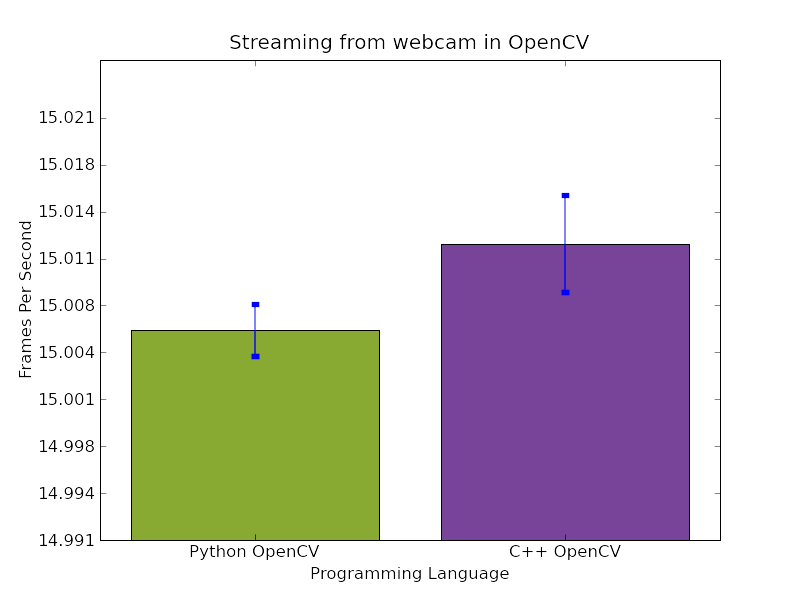
\includegraphics[width=0.95\columnwidth]{report_data/streaming_from_webcam_in_opencv}\caption{\label{fig:Streaming-comparison}Comparison of capture performances between OPENCV\_PY and OPENCV\_C.}

\end{figure}

\subsubsection*{Comparison}

Figure \ref{fig:Streaming-comparison} shows the performance results for
the previous algorithms. The measurement was done over a 2 minutes period for 3 iterations, averaging
the resulting frame rates. OpenCV Python and OpenCV C perform at very similar frame rates whilst carrying
out an I/O bound task. OpenCV C having a marginally higher frame rate output than OpenCV Python. 

The SciPy package does not currently have a direct method for image capture, so we couldn't compare live acquisition.
However, we developed a solution for using the OpenCV camera capture with SciPy: we created a Python decorator which converts the image data to a NumPy array before and after calling a Python function that processes and support NumPy images. A 640x480 RGB image takes less than 2ms to convert in either direction on the testing platform used throughout this report.

\subsection{Image Blur}

One of the simplest operations in image processing is blurring an
image. As this can be achieved in different ways, we focused here on testing a basic
Gaussian blur. As well known, this is easily achieved by convolving
the image with a Gaussian filter. Because of the separability of multidimensional
Gaussian filters \cite{young1995recursive}, the convolution can be
applied in two ways; applying a 1 dimensional filter twice, once in
each direction; or secondly the image can be convolved with a 2-dimensional
Gaussian filter created by the product of two 1 dimensional filters.

Equation \ref{eq:1D Gaussian Filter} shows the Gaussian function
for obtaining the filter in one dimension and Equation \ref{eq:2D Gaussian Filter} shows the 2 dimensional case \cite{SS01}.
 \begin{equation}
G\left(x\right)=\frac{1}{\sqrt{2\pi}\sigma}e^{-\frac{x^{2}}{2\sigma^{2}}}\label{eq:1D Gaussian Filter}\end{equation}
\begin{equation}
G\left(x,y\right)=\frac{1}{\sqrt{2\pi}\sigma^{2}}e^{-\frac{x^{2}+y^{2}}{2\sigma^{2}}}\label{eq:2D Gaussian Filter}\end{equation}
with \textit{Sigma} the standard deviation of the Gaussian distribution. 

OpenCV includes a Gaussian filter implementation that can be applied to an image by calling
the \emph{\noun{cvSmooth}} function and passing the desired filter
size. SciPy has a n-dimensional Gaussian filter that acts on a NumPy
array. Both libraries use the 1 dimensional case, as it requires less
computation.

\begin{figure}[htbp]
\begin{centering}
\subfloat[OPENCV\_C]{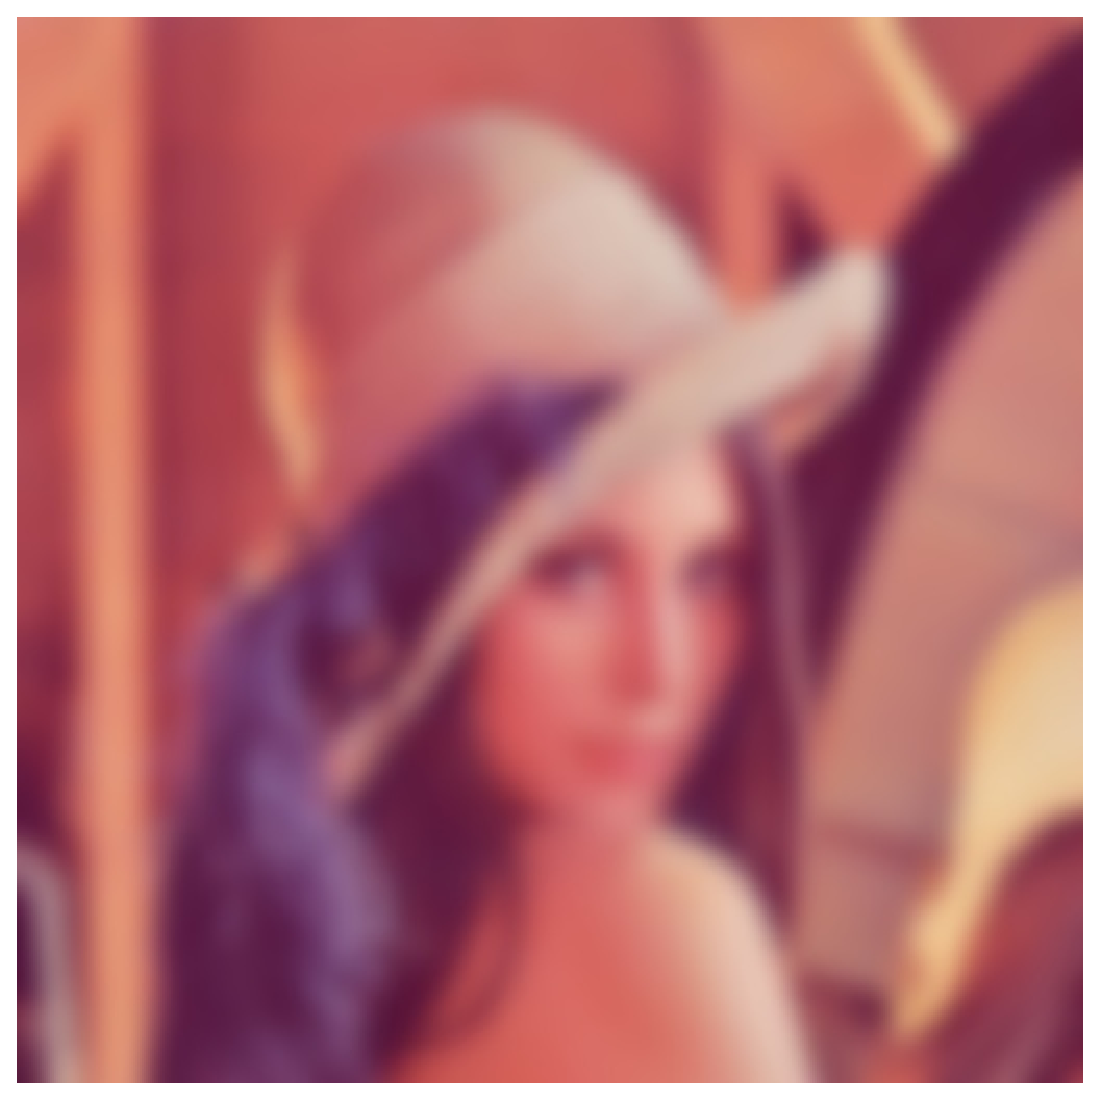
\includegraphics[width=0.33\columnwidth]{report_data/blurred_imag_cpp_opencv_gaussian}

}\subfloat[OPENCV\_PY]{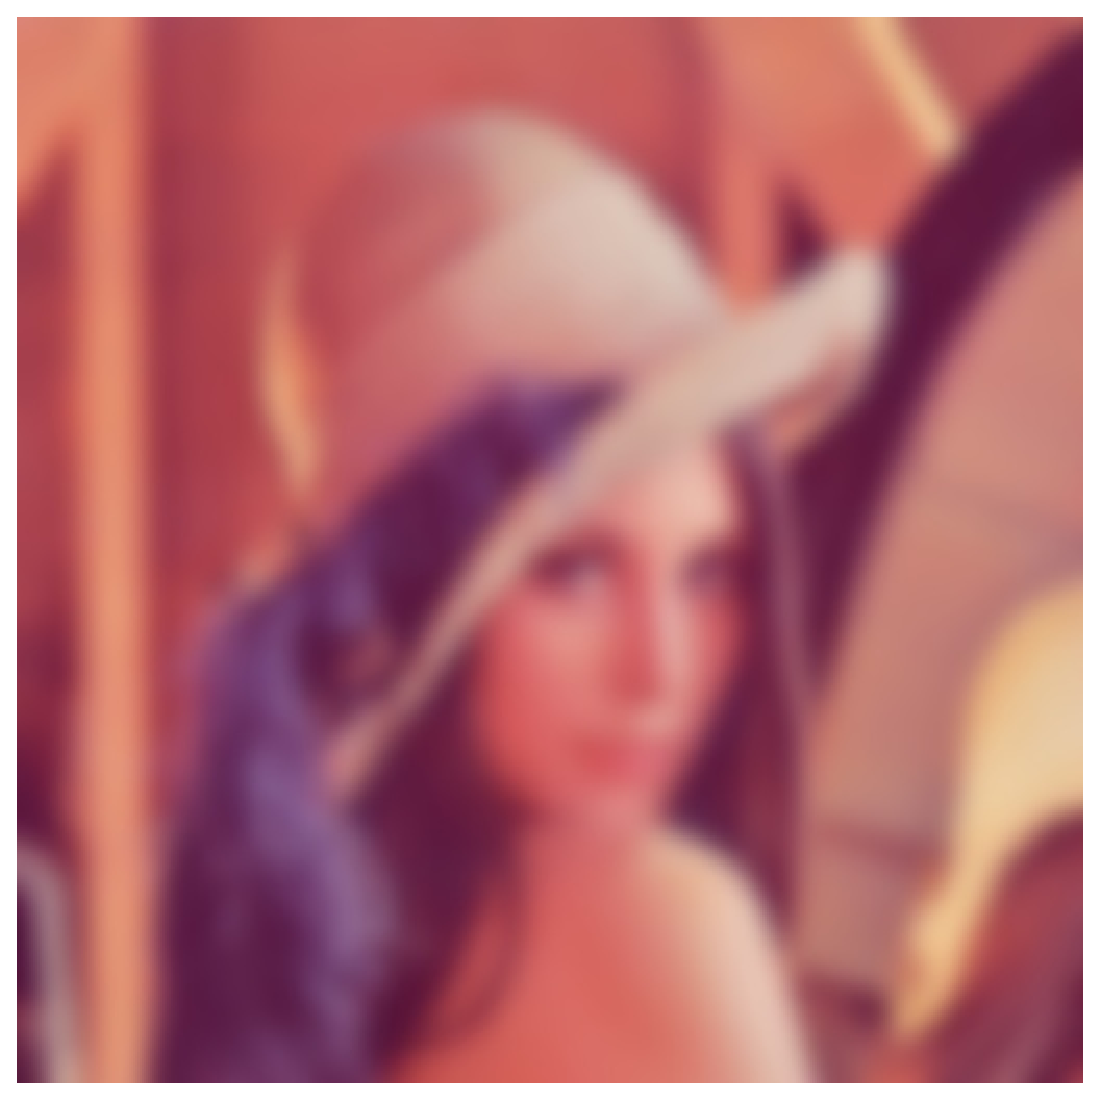
\includegraphics[width=0.33\columnwidth]{report_data/blurred_imag_python_opencv_gaussian}

}\subfloat[SCIPY]{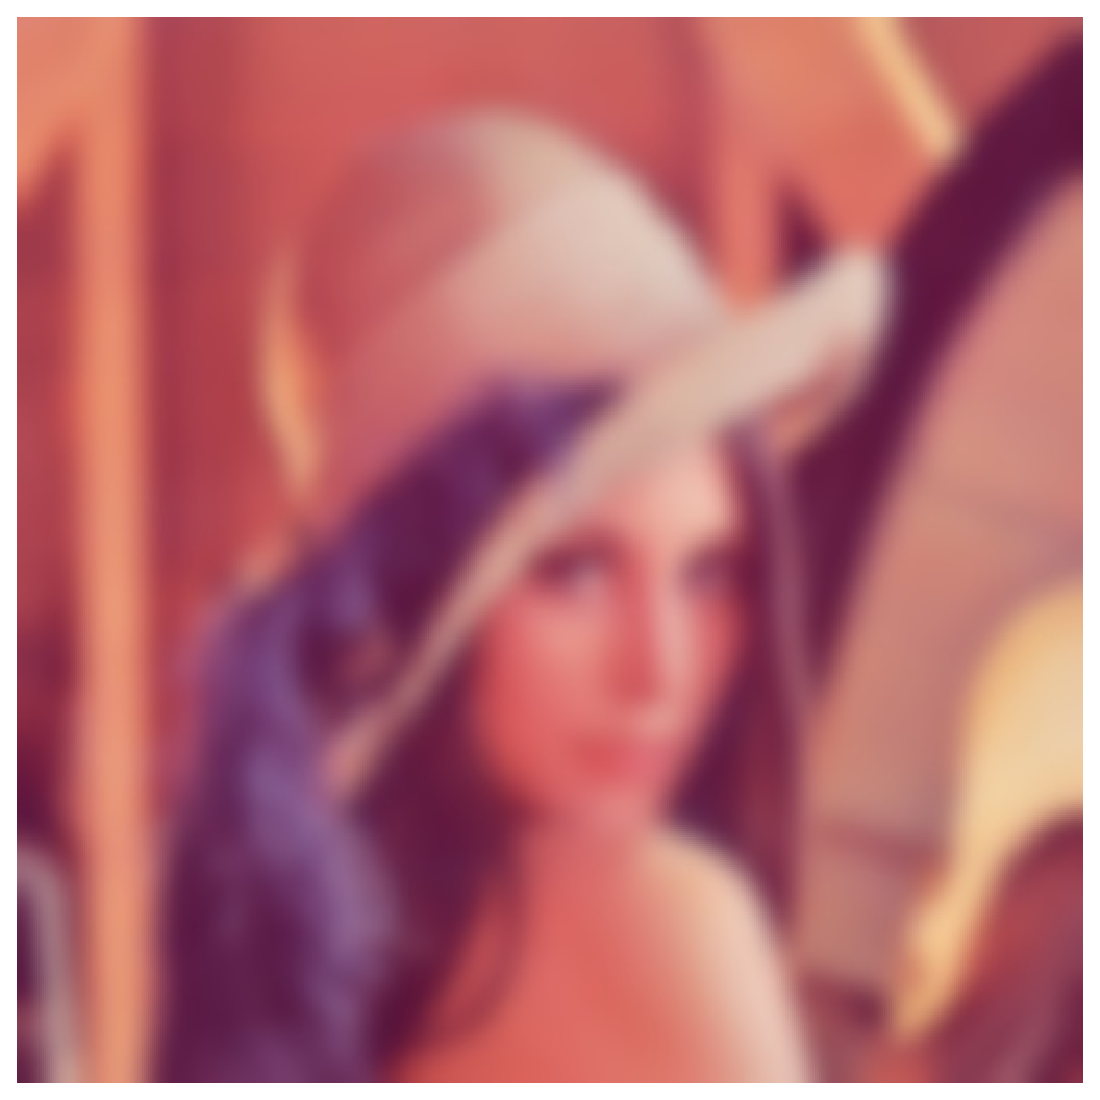
\includegraphics[width=0.33\columnwidth]{report_data/blurred_imag_python_scipy_gaussian}

}
\par\end{centering}

\caption{\label{fig:Gaussian-Output-Images}Generated Images from Gaussian Blur filter using OPENCV\_C, OPENCV\_PY and SCIPY on Lena dataset.}

\end{figure}

To ensure the same level of filtering is carried out for all the libraries, the filter parameters have been converted to be compatible with OpenCV's \noun{cvSmooth} defaults \cite{bradski2008learning}.

\subsubsection*{Comparison}

The blurred output images are shown on the Lena dataset in Figure \ref{fig:Gaussian-Output-Images}.
A basic image difference between confirmed similar results between C++/Python OpenCV version (as expected), but
small difference between SciPy and OpenCV Python code as presented Figure \ref{fig:Difference-of-each}. The graph in Figure \ref{fig:Difference-of-each} shows the pixel by pixel differences in each of the colour channels of a single image.
The maximum intensity difference at any point was 7.8\%, the mean difference was 0.8\% of the full intensity scale. 

\begin{figure}[htbp]
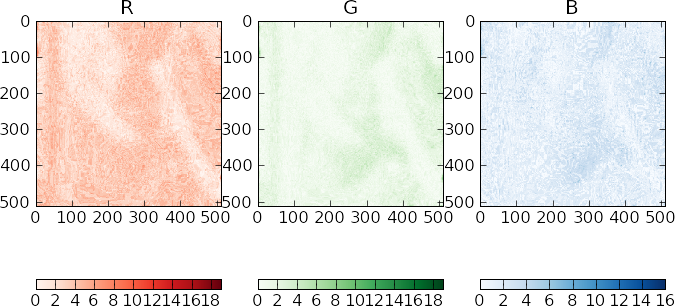
\includegraphics[width=0.98\columnwidth]{report_data/gaussian_diffs}
\caption{\label{fig:Difference-of-each} Channel Difference (RGB, 255 bits resolution) from Gaussian blur filter between OPENCV\_PY and SCIPY.}

\end{figure}

\begin{figure}[htbp]
\begin{centering}
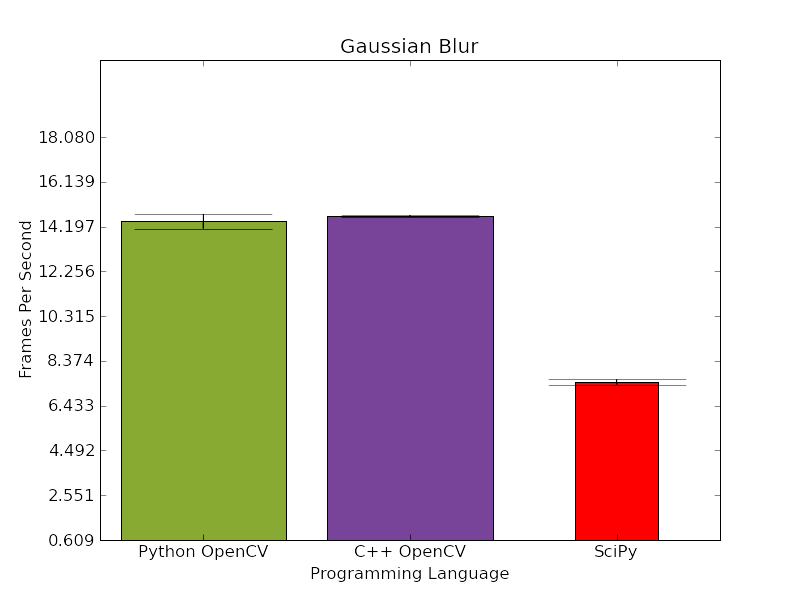
\includegraphics[width=0.9\columnwidth]{report_data/gaussian_blur}
\par\end{centering}

\caption{\label{fig:performance-gaussian}Comparison of gaussian blur performances between OPENCV\_PY, OPENCV\_C and SCIPY.}
\end{figure}
This discrepancy could be simply explained by a difference in the implementation of the
Gaussian kernel approximations. In SciPy the filter is created by
a direct sampling of the Gaussian function; OpenCV on the other hand,
uses the size of the filter, this is a good indication it probably
uses the pascal triangle as an approximation for the Gaussian kernel \cite{ben1991image}.
These differences are minor, but it is worth noting that such a simple traditionally used algorithm provides such different results.

In terms of time performance Figure \ref{fig:performance-gaussian} shows that OpenCV (either Python and C version) runs twice as fast as SciPy.
%

\subsection{Background subtraction}

A common task in security surveillance, human computer interaction is the detection of any visual changes in a video. This is done in its simplest form by a comparison of one frame to another previous frame \cite{gao2006robust}.
If the difference image is more than a certain threshold, something has changed. 

An example is presented in Figure \ref{fig:background-Adding-and-removing}
after adding a cellphone to a scene for the \noun{OPENCV\_PY} implementation. As Figure \ref{fig:BackgroundSubtract_graph} shows, the performance between Python an C are in the same order of magnitude, no significant difference were observable, where SCIPY offers inferior performances.
%
\begin{figure}[htbp]
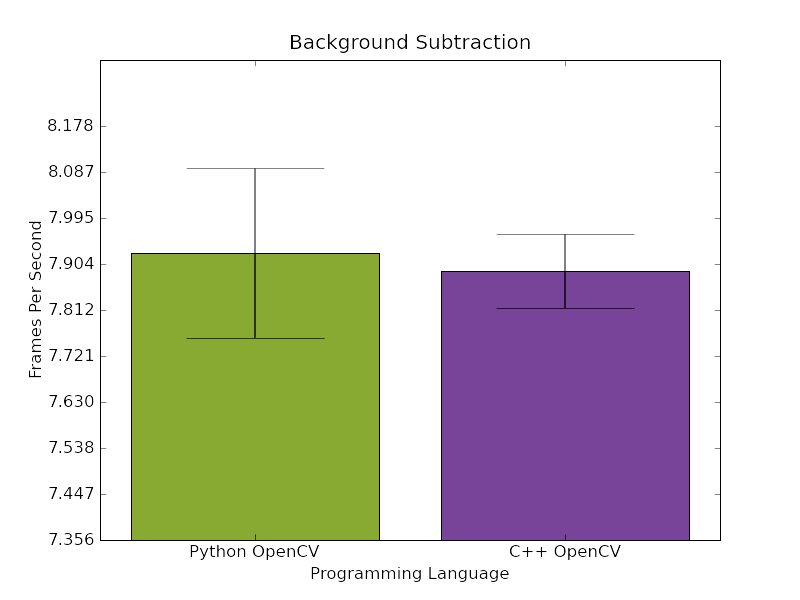
\includegraphics[width=0.95\columnwidth]{report_data/background_subtraction}

\caption{\label{fig:BackgroundSubtract_graph} Comparison of background subtraction performances between OPENCV\_PY, OPENCV\_C and SCIPY.}

\end{figure}


%
\begin{figure}[h]
\subfloat[\label{fig:Adding-a-single}Adding item]{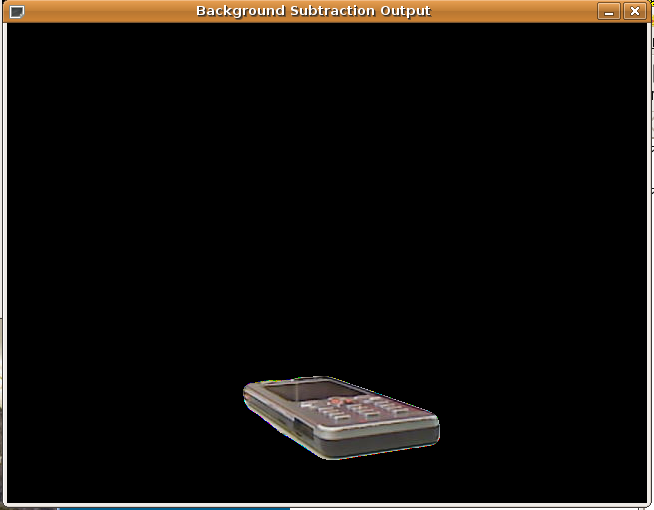
\includegraphics[width=0.33\columnwidth]{report_data/background_python_add_item}}\subfloat[\label{fig:Adding-another-item,}minor problems]{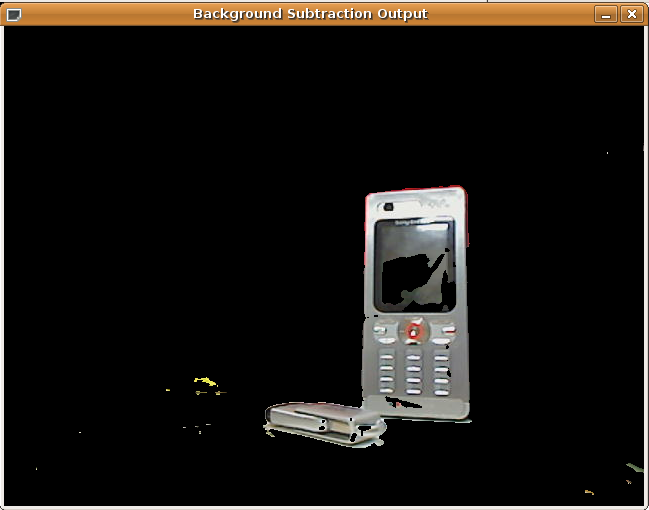
\includegraphics[width=0.33\columnwidth]{report_data/background_python_add_more_items}

}\subfloat[\label{fig:remove-laptop}Addition and removal]{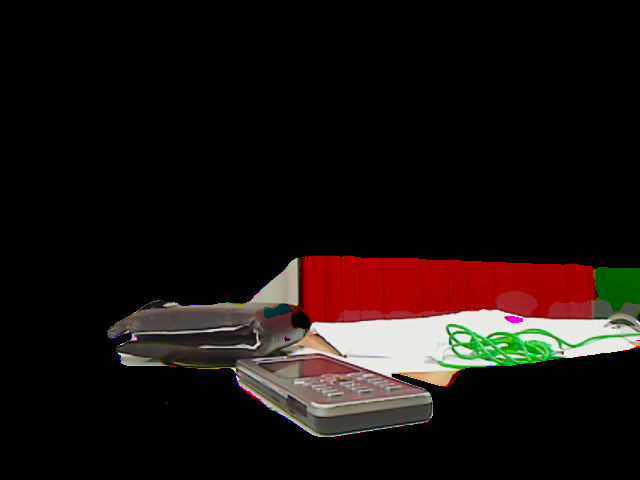
\includegraphics[width=0.33\columnwidth]{report_data/background_python_add_remove_item}

}

\caption{\label{fig:background-Adding-and-removing} Background subtraction
response after adding and removing items from a scene using OPENCV\_PY.}

\end{figure}


\subsection{Feature Point Detection}

Many methods in CV for identifying the contents of an
image rely on extracting \emph{interesting} features. Generally used as
feature points are corners of intersecting lines, line endings,
or any isolated point where local image regions have a high degree
of variation in all directions \cite{harris1988combined}. One such method
of obtaining these features is the Harris \& Stephens algorithm. According
to \cite{Sol09} the algorithm is in short: 
\begin{quote}
A matrix W is created from the outer product of the image gradient,
this matrix is averaged over a region and then a corner response function
is defined as the ratio of the determinant to the trace of W.
\end{quote}
A threshold is then applied to this corner response image to pick the most 
likely candidates and then these points are plotted. We used this algorithm 
as the basis of the test to compare the different libraries.

We took and modified an existing implementation in SciPy from \cite{Sol09}. 
A filter kernel size of 3 pixels was used when computing the harris response. 
Results are visible in Figure \ref{fig:harris_compare_static} on the Lena dataset 
for OpenCV Python and SciPy. We observed that with a larger kernel SciPy seemed
to slow down more than OpenCV. The threshold filtering and display of the corner response
was implemented solely in OpenCV to reduce differences; the SciPy
implementation therefore had an extra data conversion stage. 


\begin{figure}[h]
\begin{centering}
\subfloat[OPENCV\_PY]{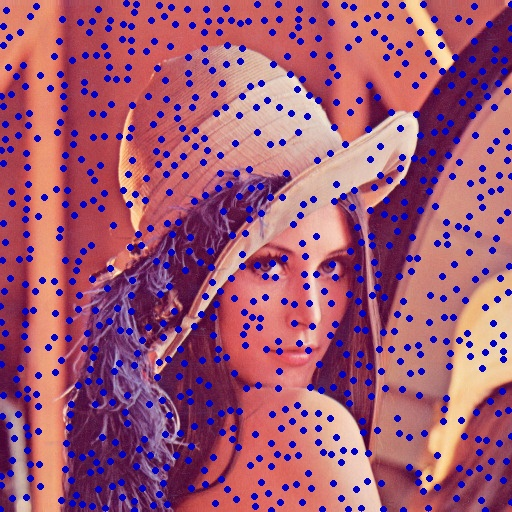
\includegraphics[width=0.455\columnwidth]{harris_response_lena_opencv}}
\subfloat[SCIPY]{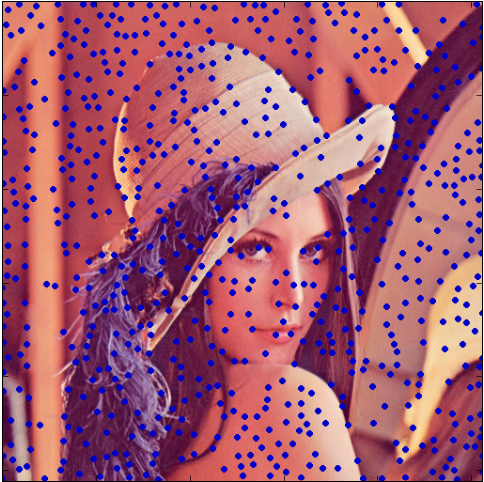
\includegraphics[width=0.45\columnwidth]{harris_scipy_static}}
\end{centering}
\caption{\label{fig:harris_compare_static}Running the Harris \& Stephens feature
detection algorithm on the Lena test image with OPENCV\_PY and SCIPY.}

\end{figure}

Visual assessment of the images show a difference of the features identified also reflecting a difference in term of implementation between both libraries. Timing performances are available on the table below (measured average over 300 iterations on the Lena dataset), OpenCV Python offering larger better performances than SciPy.
\begin{center}
\begin{tabular}{|c|c|c|}
\hline 
Library & Mean & Std\tabularnewline
\hline
\hline 
OPENCV\_PY & 65.7 ms & 1.27 ms\tabularnewline
\hline 
SCIPY & 191.5 ms & 0.87 ms\tabularnewline
\hline
\end{tabular}
\par\end{center}


\subsection{Face Detection}

Face detection is the task of identifying the presence of any number
of faces in an image, this is a specific case of general object detection.

Figure \ref{fig:OpenCV-Face-Detection} shows the output from our tests running on OpenCV Python under different conditions  using the face Haar-Cascade classifier that comes with OpenCV.

The method gave an average framerate of 7.16 \textpm{} 0.02 Hz. The
detection process itself gave very consistent timings of 107 \textpm{}
1 ms. There is no corresponding high level functionality for Face detection in SciPy, so a performance comparison was not possible. 

However, we can note that a recent project PyCV \cite{tri2009principled} improves the face detection from OpenCV utilizing SciPy.

%
\begin{figure}[h]
\subfloat[Single face in frame]{\begin{centering}
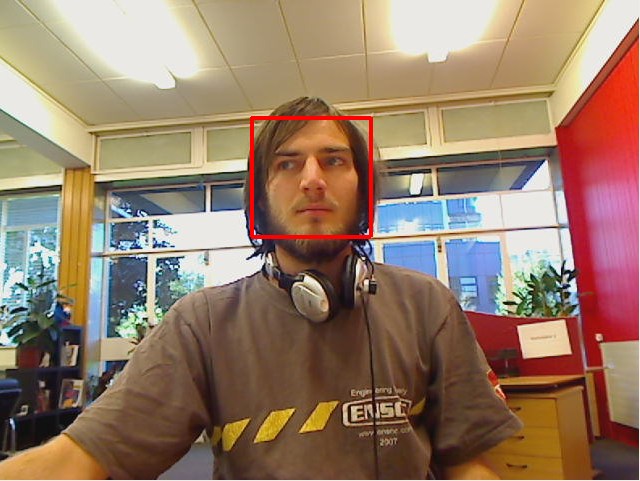
\includegraphics[width=0.455\columnwidth]{report_data/face_detect_one}
\par\end{centering}



}\subfloat[\label{fig:Obscured-opencv-face}Obscured face in frame]{\begin{centering}
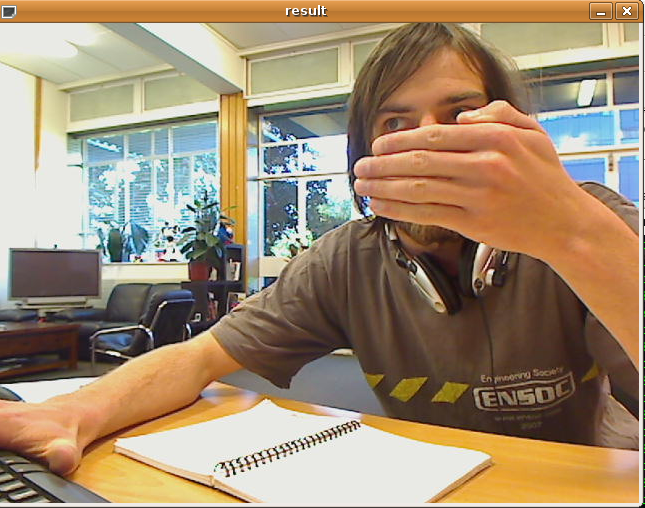
\includegraphics[width=0.45\columnwidth]{report_data/face_detect_obscure}
\par\end{centering}



}

\subfloat[Multiple faces]{\begin{centering}
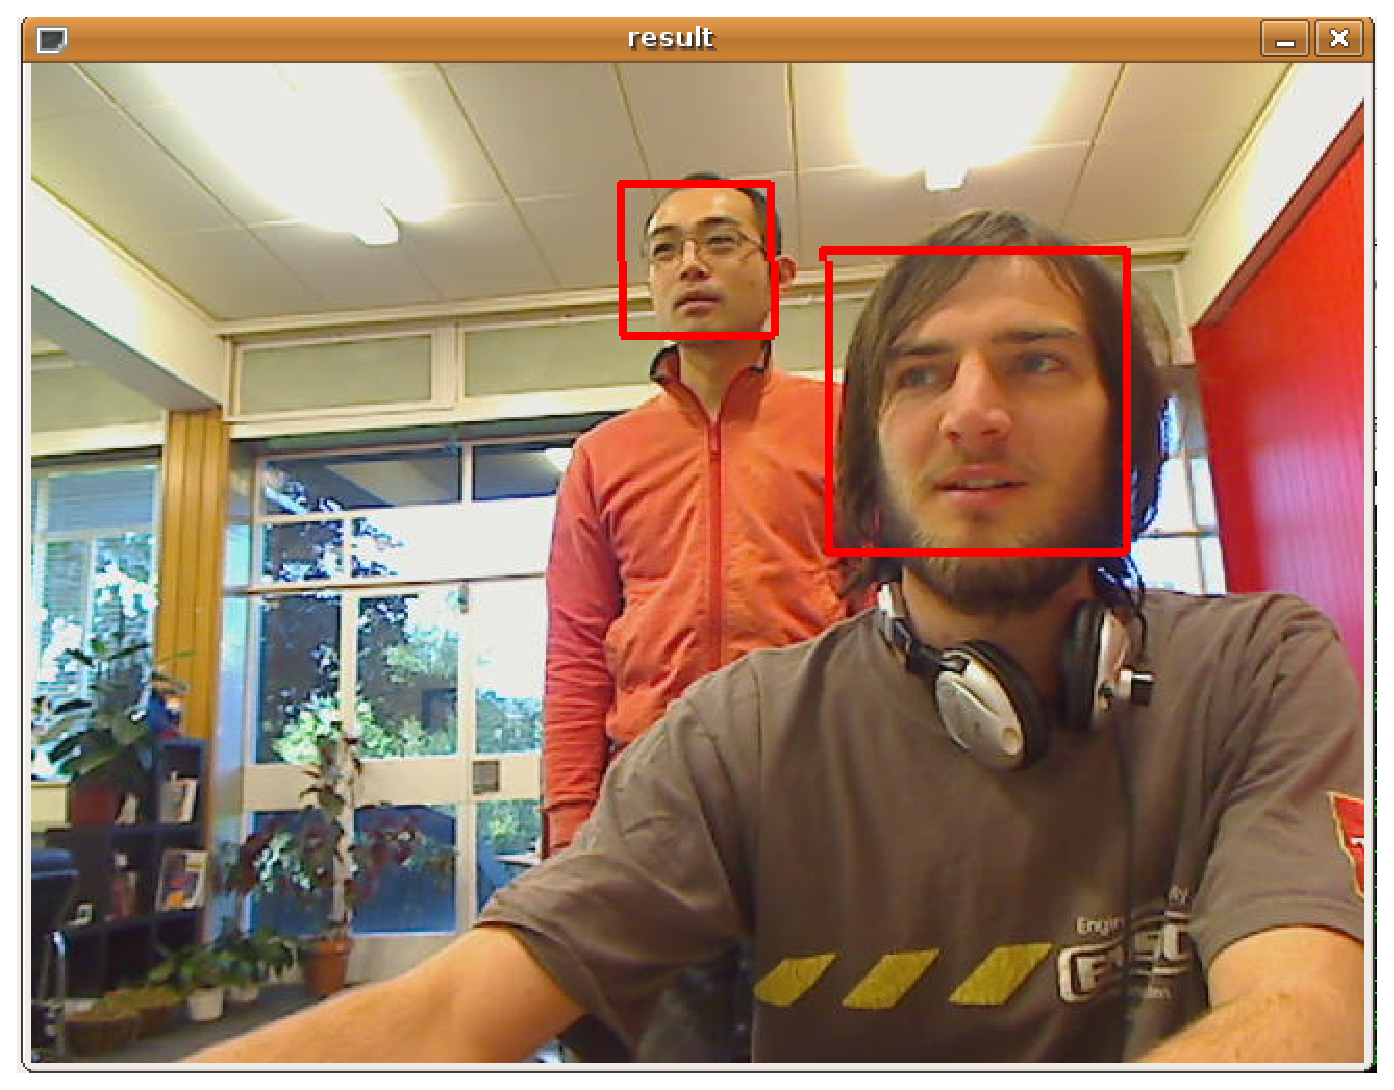
\includegraphics[width=0.45\columnwidth]{report_data/face_detect_two}
\par\end{centering}



}\subfloat[\label{fig:Angled-opencv-face}Rotated face]{\begin{centering}
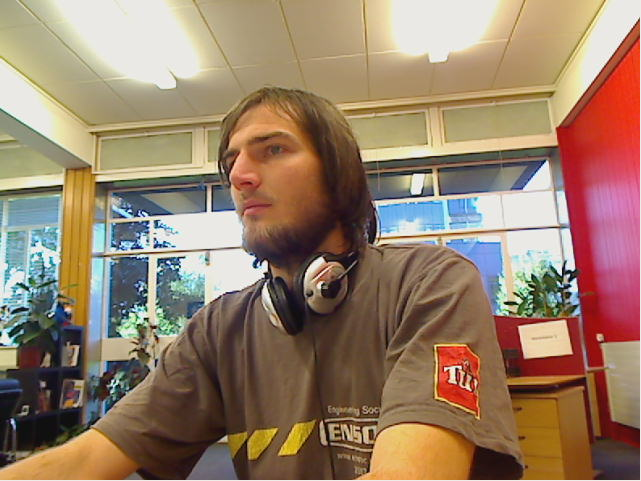
\includegraphics[width=0.45\columnwidth]{report_data/face_detect_sideways}
\par\end{centering}



}

\caption{\label{fig:OpenCV-Face-Detection}Face Detection with OPENCV\_PY}

\end{figure}


%
\section{Qualitative Comparison}

Comparing OpenCV Python vs OpenCV C, the development and testing process has been observed 
to be shorter and easier with the Python. The value of the Python interpreter as a better 
rapid prototyping tool was also quite discernible regarding the development of image 
processing/computer vision.

The documentation in both SciPy and OpenCV was found to be complete,
but not as extensive as for a professional package like MATLAB. The support
for these open source packages relies almost entirely on experienced
members of the community responding to requests on message boards
or mailing lists. The community support is however of great response and valuable technical quality.

A major limitation of using Python is the portability on embedded platforms and hardware, generally requiring
highly optimized C/C++ code.  The stability of the actual packages is also questionable: 
OpenCV Python bindings are being rewritten manually to replace the SWIG produced bindings and 
SciPy is still a relatively new library. In some cases, we also noticed the absence of analogous 
functions in both libraries, generally explained by the actual different orientation of libraries 
(SciPy more oriented for general scientific computing).

SciPy offers really valuable tools for the development and the monitoring of an application. Graphs can be generated easily with IPython based on the Matplotlib. In overall, IPython delivers pause execution during interpretation and give access to a live interactive shell with full timing and plotting capabilities (see Algorithm \ref{alg:Interactive,-inplace-timing}).
%
\begin{algorithm}
\noindent In {[}1{]}: from opencv import cv

\noindent In {[}2{]}: cv.cvAnd(diffImage,image, temp)

\noindent In {[}3{]}: timeit cv.cvAnd(diffImage,image, temp)

\noindent 1000 loops, best of 3: 229 \textmu{}s per loop

\noindent In {[}4{]}: from pylab import imshow, show

\noindent In {[}5{]}: imshow(temp) 

\noindent Out{[}5{]}: <AxesImage object at 0x42489d0>

\noindent In {[}6{]}: show()

\caption{\label{alg:Interactive,-inplace-timing} Using IPython, the interactive
shell can be used from deep inside a nested loop in a running program.
}
\end{algorithm}

Another advantage in favor of Python is its high interoperability with other libraries. For example, PyGame can be combined with OpenCV as illustrated Figure \ref{fig:Pygame-object}.

\begin{figure}
\begin{centering}
\subfloat[\label{fig:edge-filtering-face}detecting face objects]{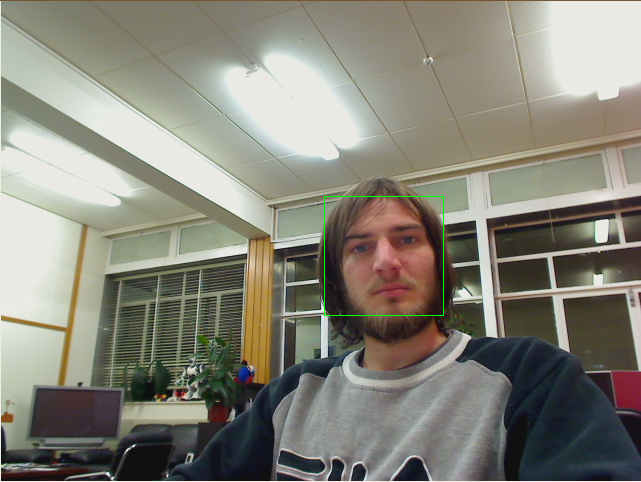
\includegraphics[width=0.49\columnwidth]{report_data/pygame-eye-locate}
}
\subfloat[edge filtering and face detection]{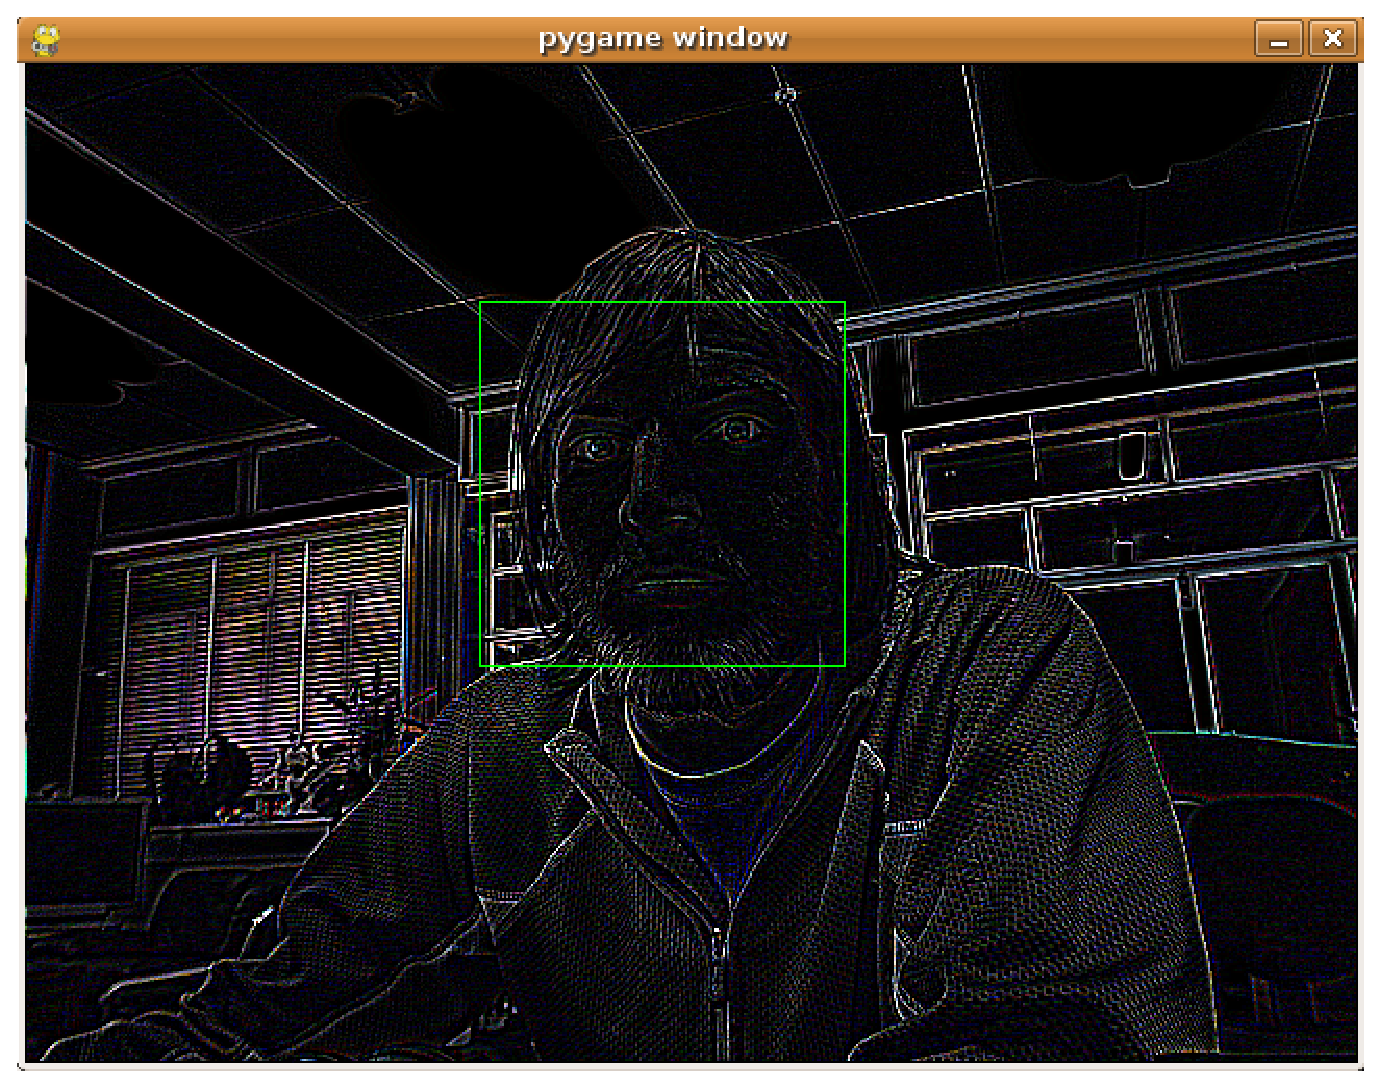
\includegraphics[width=0.49\columnwidth]{report_data/pygame-face-edge}
}
\caption{\label{fig:Pygame-object}Pygame can be used to capture and display
the video image, while OpenCV Python does the processing.}
\end{centering}
\end{figure}

\section{Related Works}

Beyond the presented libraries different works have focused on accelerating
the performances of Python interpretation.

For example, SciPy possesses the Weave module for in-lining C and C++ code that can produce code 100x faster 
than pure Python \cite{ramachandran-performance}. From a different direction a tool named \noun{OMPC} has been created for compiling MATLAB code into Python\cite{jurica2009ompc}.

For parallel programming, mixed language solutions have been shown to exhibit the same performance gains as native language solutions \cite{cai2005performance}. A different direction for parallel implementation is aimed at utilizing the power of the graphics card (GPGPU), PyGPU and the GPUCV are two examples of projects leveraging this possibility from Python \cite{lejdfors2006implementing} \cite{farrugia2006gpucv} \cite{allusse2008gpucv}.

Another related area of research is the native performance of Python itself as demonstrated by the Psyco \emph{just in time compiler} for Python \cite{rigo2004representation} (unfortunately development of this project has ceased and it is technically limited to Python 2.6.X version for x86 machines only).
We can also cite additional projects also aiming in a similar direction as:  PyPy \cite{dubois2005nest}, a compliant, flexible and fast implementation
of the Python Language, Google's \noun{Unladen
Swallow} project which aims to speed up Python by leveraging the \noun{Low
Level Virtual Machine} (LLVM). 

To finish, we can also cite Pyro \cite{blank2003pyro} a robotics simulation environment as 
another example of a platform including computer vision modules.

\section{Conclusion}

For the CV community, Python offers a valuable platform for experimenting 
new algorithms very quickly. Our tests demonstrated the quantitative and qualitative
value of Python especially regarding the OpenCV Python library. For beginners in computer vision development, we thus recommend Python. For advanced project development requiring real-time support and portability on embedded systems, OpenCV C offers a more reliable approach.

\bibliographystyle{ieeetr}
\bibliography{report_data/database}

\end{document}
